\documentclass[12pt]{article}
  
\usepackage[margin=1in]{geometry} 
\usepackage{amsmath,amsthm,amssymb,scrextend}
\usepackage{fancyhdr}
\pagestyle{fancy}
\usepackage{hyperref}

\usepackage{graphicx}
\usepackage[most]{tcolorbox}

\newcommand{\expect}[1]{\mathbb{E}\left[#1\right]}
\newcommand{\n}{\mathbf{n}}
\newcommand{\x}{\mathbf{x}}
\newcommand{\y}{\mathbf{y}}
\newcommand{\z}{\mathbf{z}}
\newcommand{\0}{\mathbf{0}}
\newcommand{\I}{\mathbf{I}}


\newcommand{\solspace}{\vspace{3mm} \textbf{Your Solution Here!} \vspace{3mm}}

\begin{document}

\lhead{ECE 551}
\chead{PSET 1 - Review and Vector spaces}
\rhead{\today}

\section{LTI Filtering - Strength of Fourier}
Suppose you have $N$ samples of a band-limited signal $x[n]$ such that, if $X = \mathcal{F}(\x)$ is the Fourier transform of $\x$, $X(\omega) = 0$ for all $\omega \geq B$. 
You have reason to believe that the signal has roughly constant magnitude within the passband, such that, in some sense, $|X(\omega)| \approx P$ where $P \in \mathbb{R}^+$ for all $\omega < B$.

The signal is corrupted with a noise vector $\n$ of  i.i.d. standard normal random variables such that $\n \sim \mathcal{N}(\0,\I)$.
The measurement available is $\y=(\x+\n) \sim \mathcal{N}(\x,\I)$.

You remember that the law of large numbers says that if you average enough well-behaved random variables, they will eventually converge to the mean, in this case, the exact signal.
Unfortunately, you only have one realization of the signal, so you decide to try using a moving average to capture some of the effect.
\vspace{3mm}

\textbf{Question: } How many points would you average? Explain your decision.
\\
How much of the noise is rejected? How much is the signal distorted?
\\
\textbf{Hint: } Recall that expectation is linear and that the signal and noise are independent. \\There isn't necessarily one correct answer.
\\
Recall the Fourier transform of a rectangular pulse is
\begin{equation}
x[n] = \begin{cases}
1, & 0 \leq n \leq M \\
0, & \text{o.w}
\end{cases} \quad
 \overset{ \mathcal{F}}{\Leftrightarrow} \quad X(\omega) = \left(\frac{\sin[\omega(M+1)/2]}{\sin(\omega/2)}\right)e^{-j\omega M/2}
\end{equation}
\solspace

\pagebreak
\section{Signal Analysis - Limitations of Fourier}
One of the nice properties of the Fourier transform is the ability to interpret the transform domain.
We have some sense of ``slow" vs ``fast" signals, hence why moving averages can be used as a heuristic to reduce the noise on certain signals.

In this problem, we'll look at two limitations of a Fourier Transform for signal analysis, in comparison to the Haar wavelet.
We will describe the Haar wavelet basis having a base length $L$ through the following equation.
\begin{equation}
\varphi (t) = \begin{cases}
\;\;\, 1, &\text{for } 0 \leq t < \frac{L}{2} \\
-1,  &\text{for } \frac{L}{2} \leq t < L \\
\quad 0,  &\text{otherwise}
\end{cases}.
\end{equation}
The additional basis vectors are defined as scaled and shifted versions by 
\begin{equation}
\varphi_{m,n} = 2^{-m/2} \varphi\left(\frac{t - n2^m}{2^m}\right).
\end{equation}
Some examples for base length 1 are included in the following figure from the text.
\begin{figure}[h]
\centering
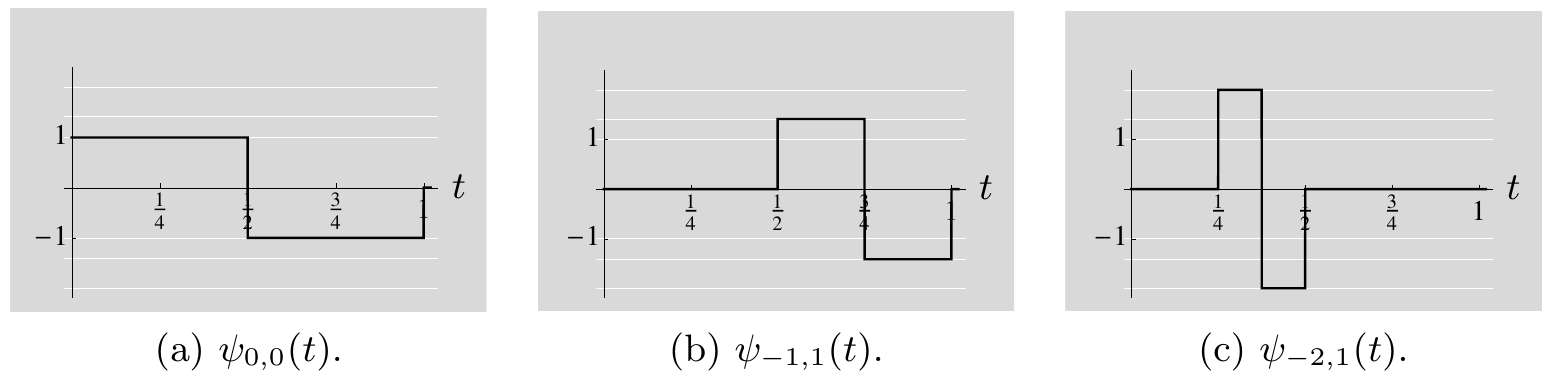
\includegraphics[width=0.8\textwidth]{haar.png}
\end{figure}

Finally, we add a constant vector $\varphi_0(t) = 1$.

(Problems on next page to avoid an unfortunate page break)

\vspace{3mm}
\pagebreak
\textbf{(a) (Multirate)} Given that the Haar Wavelet basis appears structurally similar to the Fourier basis and acquires an ability to localize high frequency changes, we will briefly consider the following set of functions
\begin{equation}
\phi (t) = \begin{cases}
\;\;\, \sin(2 \pi t), &\text{for } 0 \leq t < 1 \\
\quad 0,  &\text{otherwise}
\end{cases},
\end{equation}
where the additional scaling and shifting is defined in the same way as the Haar wavelets
\begin{equation}
\phi_{m,n} = 2^{-m/2} \phi\left(\frac{t - n2^m}{2^m}\right).
\end{equation}

\textbf{Question: } How would you represent
\begin{equation}
f(t) = 
\begin{cases}
\sin(8\pi t) + \sin(4\pi t) + \sin(2\pi t), & 0 \leq t < \frac{1}{4} \\
\sin(4\pi t) + \sin(2\pi t), & \frac{1}{4} \leq t < \frac{1}{2} \\
\sin(2 \pi t) & \frac{1}{2} \leq t < 1
\end{cases}
\end{equation}
in the set of functions  $\{\phi_{m,n}\}$? What makes the analysis of a signal into the set of functions $\{\phi_{m,n}\}$ difficult?

%Suppose you have a vector $\x_i \in \{0,1\}^2$ of length 2  for each timestep $i$ representing some underlying state of a system. This hidden state evolves in the following fashion
%\begin{equation}
%\x_{i+1} = \begin{cases}
%\begin{bmatrix}
%B_{i,1} & B_{i,2}
%\end{bmatrix}^\top \quad i \text{ is even} \\
%\begin{bmatrix}
%B_{i,1} & x_{i,2}
%\end{bmatrix}^\top \quad i \text{ is odd} \\
%\end{cases}
%\end{equation}
%where $B_{i,j}$ are Bernoulli random variables taking the values of 0 or 1 with equal probability, and $x_{i,2}$ is the second entry of $\x_i$.
%In other words, one entry potentially changes each time step, while the second can only change every other time step.\\
%Your observations come at a faster rate, generating $M$ samples between time steps of the hidden state vector, and the hidden state acts as a mask for two different periodic signals $s_1$ and $s_2$, the first of period $M$, and the second of $2M$.
%That is to say, between timesteps you observe something of the form $y_i = s_1 x_{i,1} + s_2 x_{i,2}$, where $s_2$ is one of two alternating forms. 


\solspace

\textbf{(b) (Piecewise-Constant Signals)} 

In some sense, piecewise-constant signals can be very \textit{sparse}, loosely meaning that you can fully describe the signal using very few numbers.
Unfortunately, such signals do not illustrate their sparsity in the frequency domain.
Consider the following function:
\begin{equation}
f(t) = \begin{cases}
1 & 0 \leq t - 2 k \leq \frac{1}{2} \text{ for any } k \in \mathbb{Z} \\
0 & \text{otherwise}
\end{cases}
\end{equation}
\textbf{Question:} Describe what happens to the discontinuities as you add terms in a Fourier series.
Assume a periodic extension of the Haar wavelet described earlier with a base length of 2.
How would you represent the signal in the periodic Haar basis?

\solspace


\pagebreak

\section{Inner Product Spaces Proofs}
Problem from Fall 2018 (See page 29 of VKG if you need hints)
\vspace{2mm}

(a) Prove Pythagorean Theorem

\solspace

(b) Prove Parallellogram Law

\solspace

(c) Prove Cauchy-Schwartz 

\solspace

\pagebreak
\section{A Different Type of Addition...}
Problem from Fall 2018

Let $\mathbb{R}^+$ denote the positive reals, and consider the collection 
$$
V = \left\{( x_1, x_2, ..., x_n) \mid x_k \in \mathbb{R}^+ \text{ for } k = 1, ..., n\right\}
$$
for $\x, \y \in V$ define the following summation and scaling rules:
\begin{align*}
\x + \y &:= (x_1 y_1, ..., x_n y_n) & \text{(summation)} \\
\alpha \x &:= (x_1^\lambda, ..., x_n^\lambda) & \text{(scaling)}
\end{align*}

(a) Show that $V$ is a linear space over $\mathbb{R}$ with respect to the above rules. Specify the neutral vector in $V$, and check each of the axioms individually.

\solspace

(b) Check whether the mapping $T : V \rightarrow \mathbb{R}^N$ defined below is linear. Explain your answer.
\textbf{Note: } $\mathbb{R}^N$ is the Euclidean space with standard sum and scaling.
$$
T(x) := (\log(x_1), ..., \log(x_n))
$$

\solspace

(c) Find an inner product on $V$. \\In the next homework, you will be asked to find an orthonormal basis for the space.

\solspace

\pagebreak
\section{Computational Problems - Setup}
Every problem set will have some computational problem.
This assignment is meant to make sure you have some familiarity with Python before the later assignments.

\subsection{Setup Environment}
The tools used in this assignment are
\begin{itemize} \setlength\itemsep{0.5mm}
\item Python 3 [\href{https://www.python.org/}{https://www.python.org/}]
\item IPython and Jupyter Notebook [\href{https://ipython.org/}{https://ipython.org/}]
\item Numpy [\href{https://numpy.org/}{https://numpy.org/}]
\item Matplotlib [\href{https://matplotlib.org/}{https://matplotlib.org/}]

\item Numba (Optional, but recommended) [\href{http://numba.pydata.org/}{http://numba.pydata.org/}]
\item IPywidgets (Optional, but recommended) [\href{https://ipywidgets.readthedocs.io/en/latest/}{https://ipywidgets.readthedocs.io/en/latest/}]
\end{itemize}

IPython, Numpy, Matplotlib, Numba, and IPywidgets are all libraries for Python.

Numba allows Just-In-Time (JIT) compilation of functions, and will dramatically speed up the execution of one part of the assignment, though it will run without it.

We include one interactive plot at the end of the notebook which requires ipywidgets to use, though it's not needed to complete the assignment.
\\
\\

Please familiarize yourself with the basics of Python and Numpy, as they will be used throughout the semester.
There are many tutorials available online, but here are the links to the official tutorials from the documentation.\\ \\
Python: \href{https://docs.python.org/3/tutorial/}{https://docs.python.org/3/tutorial/}\\
Numpy: \href{https://numpy.org/devdocs/user/quickstart.html}{https://numpy.org/devdocs/user/quickstart.html}

\pagebreak
\subsection{Window Functions}
For similar reasons to the effects that appear when representing discontinuities in a Fourier series, when taking some form of moving average it can sometimes be advisable to use a different \textbf{window} function.
In this problem, you will implement three different window functions. At the end of the assignment, you will qualitatively see the different behavior in when filtering and perhaps get a sense for when a more smooth window may be preferable vs. a standard rectangular window.
 
In \verb|HW1.py| please implement three functions which construct three different windows, a rectangular window, a Bartlett window, and a Hann window.
The windows should have no padding and take the entire target length, and the unnormalized forms are the following
\begin{equation}
\text{Rectangular}[n] = 1/N \quad \forall \; 0 \leq n < N
\end{equation}

\begin{equation}
\text{Bartlett}[n] = 1 - \left|\frac{2n - (N - 1)}{N-1}\right| \quad \forall \; 0 \leq n < N
\end{equation}

\begin{equation}
\text{Hann}[n] = \sin^2\left(\frac{n\pi}{N-1}\right) \quad \forall \; 0 \leq n < N
\end{equation}
where $N$ is the width of the window function.
Please normalize the windows such that the sum of the entire window is equal to 1.

The file \verb|HW1_test.py| contains some tests for both the window functions and the convolutions.
Use the flags at the top of the file to disable irrelevant tests while you're debugging.

\subsection{Circular Convolution}
While many expressions of convolution imply an infinite sequence, one method of finite-length convolution is called circular convolution.
A circular convolution is a convolution which can be thought of as convolution under periodic boundary conditions, and can be written as
\begin{equation}
(\x \circledast \y)[n] = \sum_{i=0}^{N-1} x[i] y[N + n-i \text{ mod } N]. \label{eq:conv}
\end{equation}
This form of convolution is important because it arises from the same periodicity assumption that is implicit in a Discrete Fourier Transform, and thus, while you have likely learned that convolution equates to multiplication in the frequency domain, it is in fact circular convolution through a periodic extension of the signal.\\
In \verb|HW1.py| please implement two different methods of doing a circular convolution
\begin{itemize}
\item A direct form implementing equation \ref{eq:conv}.
\item Convolution through the frequency domain using \verb|np.fft.fft| and \verb|np.fft.ifft|.
\end{itemize}

\subsection{Jupyter Notebook}
Finally, there is a Jupyter Notebook that generates some plots using your code, and includes an interactive component at the end that relates to problem 1 of the homework.
Please attach the generated plots (not including the interactive one) in your homework write-up.
Nothing else needs to be implemented, just read through the notebook.

%Every problem set will have some computational problem.
%Feel free to use whatever programming language you're familiar with, but starter code will always be provided in Julia \href{www.julialang.org}{(www.julialang.org)}, which is a programming language designed primarily for numerical and scientific computing.
%It is syntactically somewhere between Matlab and Python with a heavy emphasis on linear algebra operations.
%
%This assignment is meant to get you familiar with the basic operations that will be used heavily throughout the semester.
%There is very little independence needed for this particular problem. Just fill in some numbers and translate to the programming language you want to use.
%You will only ever be required to submit results, not the code itself.
%
%\subsection{Setup Environment}
%At this point, we'll set up the most basic requirements for the environment for the assignments.
%Make sure you have your language's equivalent.\\
%\\
%If you're setting up Julia and run into issues, feel free to email hnaumer2@illinois.edu
%\\
%\\
%The basic requirements at this point are:
%\begin{enumerate}
%\item A Programming Language
%\item Plotting
%\item Linear Algebra
%\item FFT Library
%\end{enumerate}
%Additionally, if you are using Julia/Python, you may want to install
%\begin{enumerate}
%\item Jupyter Notebooks
%\end{enumerate}
%
%\subsubsection{Programming Language Installation}
%The downloads page for Julia is \href{https://julialang.org/downloads/}{https://julialang.org/downloads/}.
%\\
%
%\textbf{Linux}: \\You likely you know what to do for your system better than I do.
%An unofficial binary of Julia is most likely available in your package manager under a name like ``julia."
%They recommend using the official binary, but so far I haven't had a problem using the unofficial one for my platform.
%\\
%
%\textbf{Windows or Mac}: \\There is an installer on the downloads page. You may need to add Julia to your path. 
%\\
%Additional information is available here: \href{https://julialang.org/downloads/platform/}{https://julialang.org/downloads/platform/}
%\vspace{1cm}
%\\
%Open a terminal and run the command \verb|julia| to open the REPL.
%
%\subsubsection{Plotting Library}
%Julia has a package manager built in, so installing libraries is very simple.
%
%First, open the REPL in a terminal by running the command \verb|julia|
%\begin{verbatim}
%[helmuth@naumer ~]$ julia
%
%               _
%   _       _ _(_)_     |  Documentation: https://docs.julialang.org
%  (_)     | (_) (_)    |
%   _ _   _| |_  __ _   |  Type "?" for help, "]?" for Pkg help.
%  | | | | | | |/ _` |  |
%  | | |_| | | | (_| |  |  Version 1.5.0 (2020-08-01)
% _/ |\__'_|_|_|\__'_|  |  
%|__/                   |
%
%julia> 
%
%\end{verbatim}
%
%Once the REPL is open, type the key \verb|]| to enter the package manager mode.
%\begin{verbatim}
%(@v1.5) pkg>
%\end{verbatim}
%
%The easiest plotting library is \href{http://docs.juliaplots.org/latest/}{Plots.jl}.
%Install it by typing \verb|add Plots|, which should output the following with many other dependencies installed after.
%\begin{verbatim}
%(@v1.5) pkg> add Plots
%   Updating registry at `~/.julia/registries/General`
%  Resolving package versions...
%Updating `~/.julia/environments/v1.5/Project.toml`
%  [91a5bcdd] + Plots v1.6.0
%Updating `~/.julia/environments/v1.5/Manifest.toml`
%\end{verbatim}
%
%Now let's test the installation real quick. Hit backspace to leave the package manager and import the plotting library with \verb|using Plots|.
%This will take a while because it does some compilation operations the first time a library is imported.
%\begin{verbatim}
%julia> using Plots
%[ Info: Precompiling Plots [91a5bcdd-55d7-5caf-9e0b-520d859cae80]
%\end{verbatim}
%
%Now try plotting $y = x^2$. \\The first plot each time Julia is run is also slow due to the compilation paradigm.
%\begin{verbatim}
%julia> x = 0:0.01:1;
%
%julia> plot(x,x.^2,label="",linecolor=:black)
%
%julia> 
%\end{verbatim}
%
%\subsubsection{Linear Algebra}
%In Julia, most likely all needed linear algebra operations are built into the standard libraries.
%If you're using Python, numpy will make your life easier.
%
%\subsubsection{DFT Library}
%FFTW (\href{http://www.fftw.org/}{http://www.fftw.org/}), or ``The Fastest Fourier Transform in the West" is one of the standard Fourier transform library with wrappers available in most languages and is used behind the scenes in places like MATLAB.
%You just need some way to compute Fourier transforms of vectors in $\mathbb{C}^N$, it may not be called FFTW.
%It is not advisable to just naively implement a DFT, or even the standard Cooley-Tukey FFT algorithm.
%
%In Julia, the library is installed by entering the package manager again with \verb|]| and running
%\begin{verbatim}
%(@v1.5) pkg> add FFTW
%\end{verbatim}
%
%\subsubsection{Jupyter Notebook}
%Install the IJulia kernel for Jupyter.
%If Jupyter is not already installed, running IJulia will automatically install a small Python + Jupyter setup private to Julia.
%\begin{verbatim}
%(@v1.5) pkg> add IJulia
%\end{verbatim}
%
%Hit backspace to leave the package manager and run
%\begin{verbatim}
%julia> using IJulia
%[ Info: Precompiling IJulia [7073ff75-c697-5162-941a-fcdaad2a7d2a]
%
%julia> notebook()
%\end{verbatim}
%
%At this point, it should guide you through the rest of the installation and then open in your default web browser.
%
%\subsubsection{Exit REPL}
%At this point, exit the REPL by running
%\begin{verbatim}
%julia> exit()
%\end{verbatim}
%
%Note that this will end the Jupyter session that was previously started.


\end{document}